\documentclass[tikz,border=2pt]{standalone}
\usepackage{amsmath}
\usepackage{pgfplots}
\pgfplotsset{compat=1.18}
\usetikzlibrary{arrows.meta}
\begin{document}
% Complementary slackness on Example 5.1: at x*=(2,6) the constraints 2x2<=12 and 3x1+2x2<=18 are binding
% (y2*=3/2>0, y3*=1>0); x1<=4 has slack 4-2=2, so y1*=0. Objective line 3x1+5x2=36 touches the region at x*.
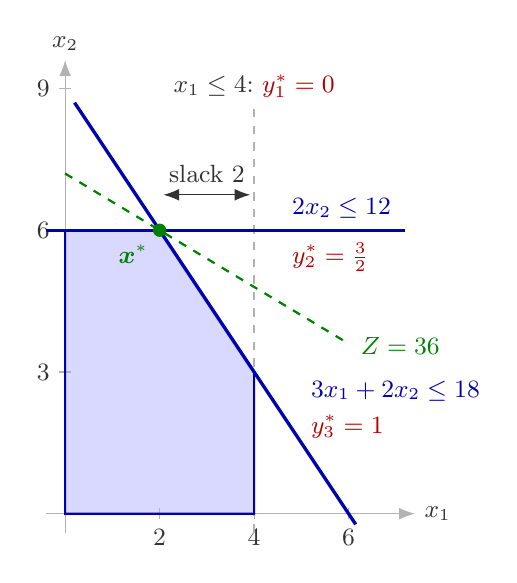
\begin{tikzpicture}[font=\small, >={Latex[length=2mm]}, x=0.6cm, y=0.6cm]
  % feasible region
  \fill[blue!15] (0,0) -- (4,0) -- (4,3) -- (2,6) -- (0,6) -- cycle;
  % axes
  \draw[gray!60, ->] (-0.4,0) -- (7.4,0) node[anchor=west, gray!40!black] {$x_1$};
  \draw[gray!60, ->] (0,-0.4) -- (0,9.6) node[anchor=south, gray!40!black] {$x_2$};
  \foreach \t in {2,4,6} {
    \draw[gray!60] (\t,0.12) -- (\t,-0.12);
    \node[gray!40!black, anchor=north] at (\t,-0.12) {$\t$};
  }
  \foreach \t in {3,6,9} {
    \draw[gray!60] (0.12,\t) -- (-0.12,\t);
    \node[gray!40!black, anchor=east] at (-0.12,\t) {$\t$};
  }
  % nonbinding constraint x1 <= 4
  \draw[gray!60, dashed, thick] (4,-0.4) -- (4,8.6);
  \node[gray!40!black, anchor=south] at (4,8.6) {$x_1\leq4$:\ \textcolor{red!70!black}{$y_1^{\ast}=0$}};
  % binding constraints at x*
  \draw[blue!70!black, very thick] (-0.4,6) -- (7.2,6);
  \node[blue!70!black, anchor=south west] at (4.6,6.05) {$2x_2\leq12$};
  \node[red!70!black, anchor=north west] at (4.6,5.95) {$y_2^{\ast}=\tfrac{3}{2}$};
  \draw[blue!70!black, very thick] (0.2,8.7) -- (6.15,-0.225);
  \node[blue!70!black, anchor=west] at (5.0,2.6) {$3x_1+2x_2\leq18$};
  \node[red!70!black, anchor=west] at (5.0,1.85) {$y_3^{\ast}=1$};
  % region boundary
  \draw[blue!70!black, thick] (0,0) -- (4,0) -- (4,3) -- (2,6) -- (0,6) -- cycle;
  % objective line through x*
  \draw[green!50!black, thick, dashed] (0,7.2) -- (6,3.6);
  % slack of the first constraint
  \draw[gray!40!black, <->] (2.08,6.75) -- (3.92,6.75);
  \node[gray!40!black, anchor=south] at (3,6.8) {slack $2$};
  % optimum
  \fill[green!50!black] (2,6) circle (2.4pt);
  \node[green!50!black, anchor=north east] at (1.95,5.9) {$\boldsymbol{x}^{\ast}$};
  \node[green!50!black, anchor=west] at (6.05,3.55) {$Z=36$};
\end{tikzpicture}
\end{document}
